\newpage
\section{Interprétation }
\subsection{Évolution de la fonction coût et distance d'édition:}

    La figure suivante représente l'évolution de la fonction de coût et de la distance de Levenstein de notre réseau au cours de l'entraînement de la validation pour 100 époques.
    
    \begin{figure}[!ht]
        \centering
        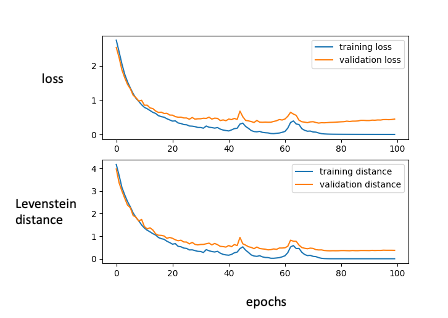
\includegraphics[width=120mm]{sections/images/interpretation/bidirLoss.png}
        \caption{Évolution de la fonction de coût et de la distance}
        \label{fig:Figure 10  }
    \end{figure}
    
    \subsubsection{Interprétation de la fonction de coût}
        Au cours de premières itérations nous pouvons observer une décroissance rapide de la fonction de coût pour la validation et l'entraînement. La fonction de coût se stabilise entre 30 et 70 itérations avec l'apparition de quelques sauts. Enfin, vers la 70ème itération nous remarquons un sur-apprentissage du réseau car nous arrivons à annuler complètement la fonction de coût pour l'entraînement alors qu'elle commence à remonter pour la validation.
        Le réseau n'étant plus en mesure de généraliser correctement nous gardons le modèle ayant la meilleure distance en validation.

    \subsubsection{Interprétation de la fonction de la distance de Levenstein}
        La distance moyenne de Levenstein suit la même évolution que la fonction de coût et nous pouvons observer les mêmes phénomènes de sur-apprentissages qu'avec la fonction de coût. Notre réseau arrive à obtenir une distance moyenne nulle en entraînement et arrive à descendre à environ 0.35 de distance en validation. Ces résultats sont corrects car ils signifient qu'en moyenne notre réseau se trompe sur moins d'une lettre.



\subsection{Matrice de confusion :}
    Une fois le réseau entraîné nous obtenons pour 100 mots pris au hasard la matrice de confusion normalisée suivante :
    \begin{figure}[!ht]
        \centering
        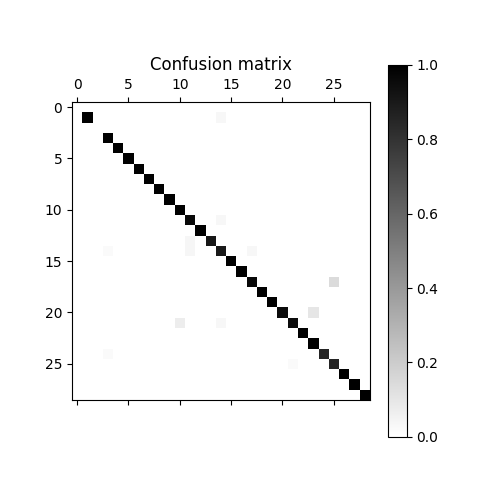
\includegraphics[width=120mm]{sections/images/interpretation/bidir matrix.png}
        \caption{Matrice de confusion pour 100 mots}
        \label{fig:Figure 11  }
    \end{figure}
    La matrice de confusion suivante possède en ordonné les indexes des symboles cibles et en abscisse les indexes des symboles prédits. 
    Pour chaque mot nous cumulons ces valeurs dans la matrice puis nous normalisons par rapport à la somme des valeurs cibles de chaque symbole sur les lignes de la matrice afin d'avoir une représentation sous forme de fréquence d'apparition (entre 0 et 1). De plus, nous ignorons l'apparition du symbole de 'départ de séquence' car il n'apparaît pas, ainsi que du 'remplissage' car il est traité en amont et ignoré pendant l'apprentissage. Enfin nous pouvons commenter que les résultats présentés par la matrice sont très bons car nous observons une haute fréquence d'apparition des symboles cibles et prédits. C'est à dire par la présence d'une diagonale avec des valeurs proches de 1.
    
    


\subsection{Représentation de l'attention :}
    Pour chaque lettre prédite nous pouvons récupérer les poids d'attentions afin d'observer sur quelle partie de la séquence le réseau met l'emphase.
    \newline Sans bidirectionnalité nous obtenions les résultats suivants :
    \begin{figure}[!ht]
        \centering
        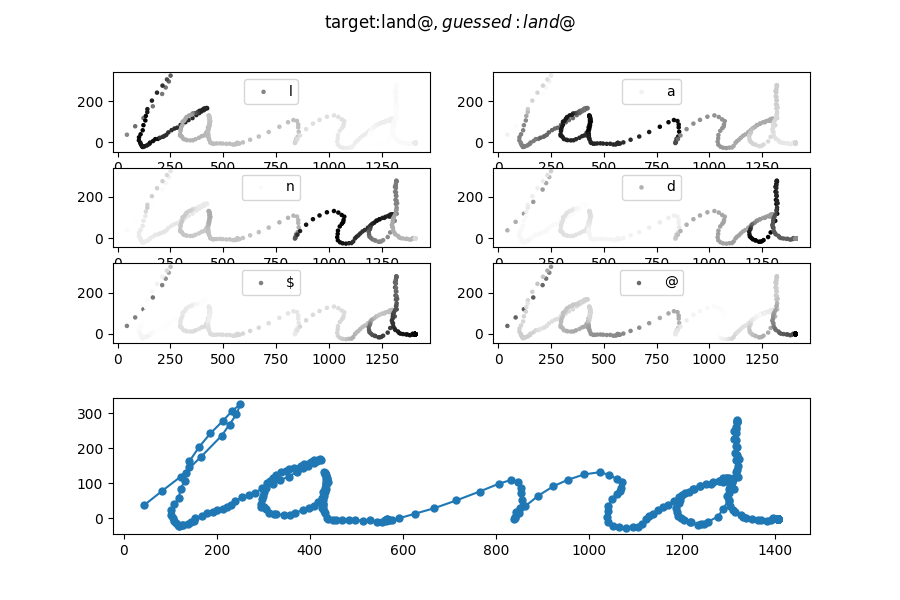
\includegraphics[width=120mm]{sections/images/interpretation/lastGRUatt2.png}
        \caption{Affichage de l'attention sans bidirectionnalité}
        \label{fig:Figure 12  }
    \end{figure}
    
    Avec bidirectionnalité nous obtenons les résultats suivants :
    
    \begin{figure}[!ht]
        \centering
        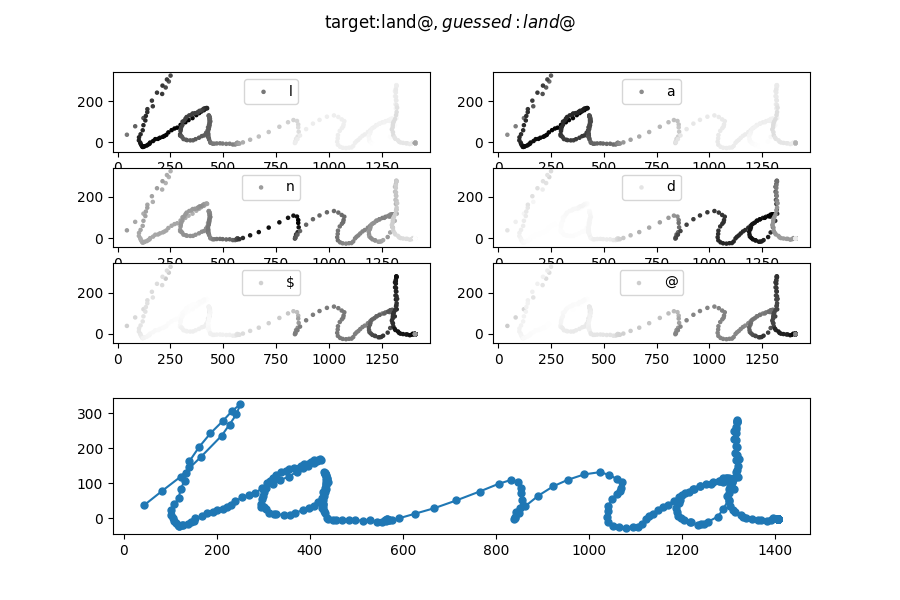
\includegraphics[width=120mm]{sections/images/interpretation/bidirtest2.png}
        \caption{Affichage de l'attention avec bidirectionnalité}
        \label{fig:Figure 13  }
    \end{figure}
     Comme voulu, l'attention permet de porter l'emphase sur la partie de la séquence à traduire. Néanmoins nous pouvons observer une différence avec et sans bidirectionnalité. Lorsque cette dernière n'est pas présente le réseau semble porter son attention sur la fin de la séquence représentant la lettre. Par exemple sur la figure (\ref{fig:Figure 12  }) nous pouvons voir que nous nous concentrons sur la fin de la lettre n sans bidirectionnalité alors que nous prenons en un contexte content la lettre en entier lorsque la bidirectionnalité est activée sur la figure (\ref{fig:Figure 13  }). Nous pouvons conclure que la bidirectionnalité est donc bénéfique pour l'attention avec elle permet d'avoir un contexte plus précis du mot en explorant en avant et en arrière la séquence.
    
    
    

\subsection{Traduction avec le sous-ensemble test :}

    En testant plusieurs cas du sous-ensemble de test nous obtenions des résultats corrects. Le réseau arrivait à traduire correctement la séquence avec en moyenne moins d'une lettre d'erreur comme pour la validation.
    \begin{figure}[!ht]
        \centering
        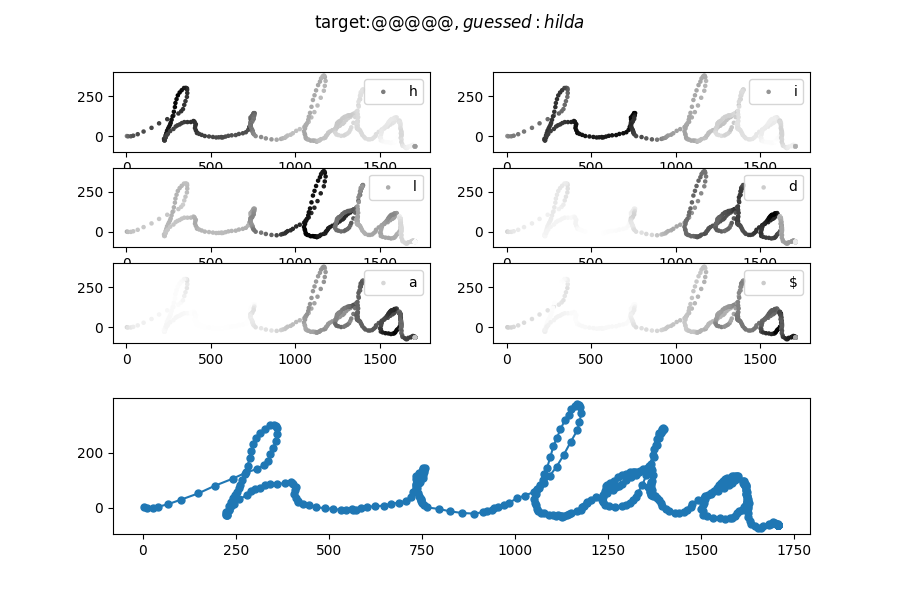
\includegraphics[width=120mm]{sections/images/interpretation/TEST_attention.png}
        \caption{Affichage de l'attention avec bidirectionnalité avec le sous ensemble de test}
        \label{fig:Figure 14  }
    \end{figure}